\documentclass{standalone}
\usepackage{tikz}
\usetikzlibrary{calc}
\begin{document}
    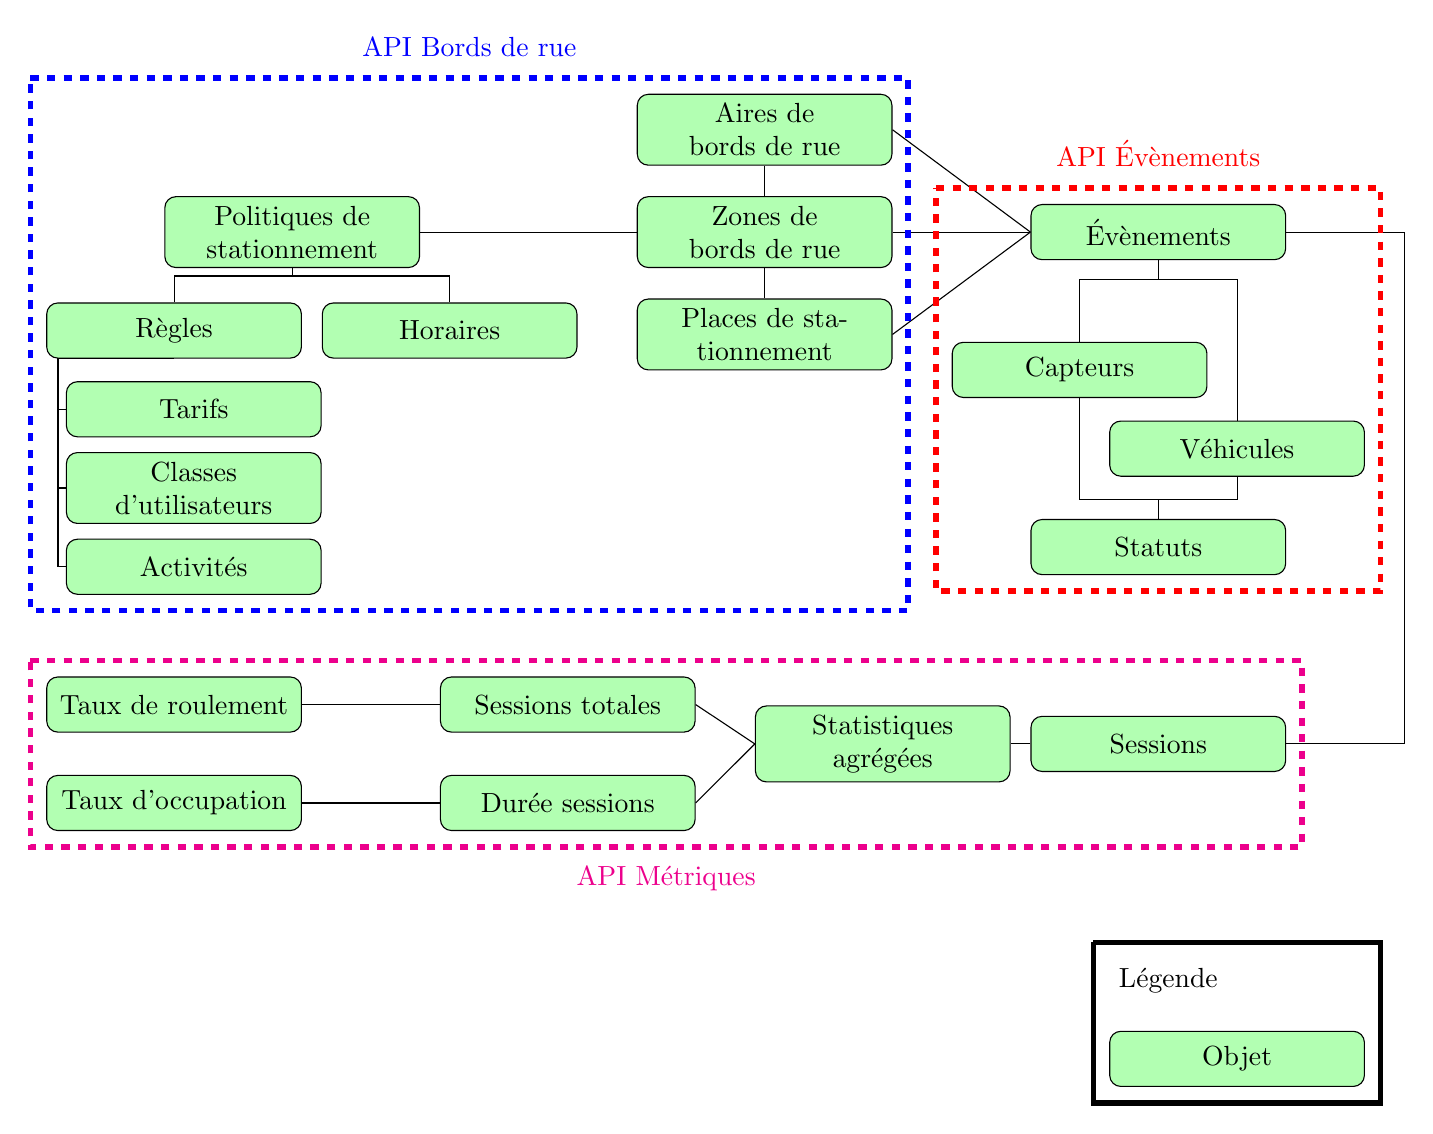
\begin{tikzpicture}
        \tikzstyle {objet} = [rectangle, rounded corners, text width=3cm, minimum height=0.7cm,text centered,  draw=black, fill=green!30]
        \tikzstyle {propriete} = [rectangle, rounded corners, text width=3cm, minimum height=0.7cm,text centered,  draw=black, fill=orange!30]
        % Évènements
        \node (status) [objet]{Statuts};
        \node (capteurs) [objet,above of=status,xshift=-1cm,yshift=1.25cm]{Capteurs};
        \node (vehicules) [objet, above of=status,xshift=1cm,yshift=0.25cm]{Véhicules};
        \draw (status.north) |- ++(0,0.25) -| (capteurs.south);
        \draw (status.north) |- ++(0,0.25) -| (vehicules.south);
        \node (evenements) [objet,above of=status,yshift = 3cm]{Évènements};
        \draw (evenements.south) |- ++(0,-0.25) -| (capteurs.north) ;
        \draw (evenements.south) |- ++(0,-0.25) -| (vehicules.north);
        
        % BDR
        \node (zones) [objet,left of=evenements,xshift=-4cm]{Zones de bords de rue};
        \draw (evenements.west) -> (zones.east);
        \node (area) [objet, above of=zones,yshift=0.3cm]{Aires de bords de rue};
        \draw (area.south) -> (zones.north);
        \draw (evenements.west)->(area.east);
        \node (spaces) [objet, below of=zones,yshift=-0.3cm]{Places de stationnement};
        \draw (spaces.north) -> (zones.south);
        \draw (evenements.west)->(spaces.east);
        \node (politiques) [objet, left of=zones,xshift=-5cm]{Politiques de stationnement};
        \draw (zones.west)->(politiques.east);
        \node (regles) [objet, below of=politiques,xshift=-1.5cm,yshift=-0.25cm]{Règles};
        \draw (politiques.south) |- ++(-0.1cm,-0.1cm) -| (regles.north);
        \node (horaires) [objet, right of=regles,xshift=2.5cm]{Horaires};
        \draw (politiques.south) |- ++(0.1cm,-0.1cm) -| (horaires.north);
        \node (tarifs) [objet, below of=regles,xshift=0.25cm] {Tarifs};
        \draw (tarifs.west) -| ++(-0.1cm,0.1cm) |-(regles.south);
        \node (classes_utilisateurs) [objet,below of=tarifs]{Classes d'utilisateurs};
        \draw (tarifs.west) -| ++(-0.1cm,-0.1cm) |-(classes_utilisateurs.west);
        \node (activite) [objet,below of=classes_utilisateurs]{Activités};
        \draw (classes_utilisateurs.west) -| ++(-0.1cm,-0.1cm) |- (activite.west);
        % Métrique
        \node (sessions) [objet,below of=status,yshift=-1.5cm]{Sessions};
        \node (aggregates) [objet, left of=sessions, xshift=-2.5cm]{Statistiques agrégées};
        \draw (sessions.west) -- (aggregates.east);
        \node (total_session) [objet, left of=aggregates,xshift=-3cm,yshift=0.5cm]{Sessions totales};
        \draw (aggregates.west) -- (total_session.east);
        \node (taux_roulement)at ($ (regles |- total_session) $) [objet]{Taux de roulement};
        \draw (taux_roulement.east) -- (total_session.west);
        \node (dwell_time) [objet,below of=total_session,yshift=-0.25cm]{Durée sessions};
        \draw (dwell_time.east) -- (aggregates.west);
        \node (taux_occupation) at ($ (taux_roulement |- dwell_time) $) [objet]{Taux d'occupation};
        \draw (taux_occupation.east) -- (dwell_time.west);
        \draw (evenements.east) -| ++(1.5cm,-2cm) |- (sessions.east);
        % Légende
        \node (legend) [below of=sessions, text width=3cm,xshift=1cm,yshift=-2cm]{Légende};
        \coordinate (boite_top_left)at($(legend.north west)+ (-0.2,0.2)$);
        \node (objet_desc)[objet,below of=legend]{Objet};
        \coordinate (boite_bot_rght) at ($(objet_desc.south east)+ (0.2,-0.2)$);
        \draw[line width=2pt] (boite_top_left) -| (boite_bot_rght) -| (boite_top_left);
        % API domaines
        % Évènements
        \coordinate (events_top_left) at ($(evenements.north -| capteurs.west)+ (-0.2,0.2)$);
        \coordinate (events_bottom_right) at ($(status.south -| vehicules.east)+ (0.2,-0.2)$);
        \draw[dashed, line width=2pt, red] (events_top_left) -| (events_bottom_right) -| (events_top_left);
        \node (label_events_api) [above of=evenements,color=red]{API Évènements};
        % Bords de rue
        \coordinate (bdr_top_left) at ($(area.north -| regles.west) + (-0.2,0.2)$);
        \coordinate (bdr_bottom_right) at ($(activite.south -| area.east) + (0.2,-0.2)$);
        \coordinate (bdr_top_center) at ($(bdr_top_left)!0.5!(bdr_top_left -| bdr_bottom_right)$);
        \draw[dashed, line width=2pt, blue] (bdr_top_left) -| (bdr_bottom_right) -| (bdr_top_left);
        \node (label_curbs_api) at ($(bdr_top_center) + (0,0.4)$) [color=blue] {API Bords de rue};
        % metriques
        \coordinate (metriques_haut_gauche) at ($(taux_roulement.north west) + (-0.2,0.2)$);
        \coordinate (metriques_bas_droite) at ($ (taux_occupation.south -| sessions.east) + (0.2,-0.2)$);
        \coordinate (metriques_bas_centre) at ($(metriques_bas_droite)!0.5!(metriques_bas_droite -| metriques_haut_gauche)$);
        \draw[dashed, line width=2 pt, magenta] (metriques_haut_gauche)-| (metriques_bas_droite) -| (metriques_haut_gauche);
        \node (label_metriques_api) at ($(metriques_bas_centre) + (0,-0.4)$) [color=magenta] {API Métriques};
    \end{tikzpicture}
\end{document}